\section{Curriculum Proposal}

The primary concerns addressed in Chapter 1 are as follows:

\begin{enumerate}
    \item Students lack a solid foundation in the fundamentals of programming.
    \item Programming is an under utilized problem-solving technique in the Department of Mechanical
    Engineering at K-State.
\end{enumerate}
To address the first issue, two proposals are made: the adoption of a single programming 
language and the restructuring of programming classes in the department. First, the goal of adopting a single 
programming language is to give students a more thorough understanding in a single language rather than 
a shallow understanding of four languages. The language chosen in this project is Python. In conjunction with 
Python, a consistent environment should be used as well. A consistent environment will prevent unnecessary 
confusions from IDE specific features and setup requirements. The chosen environment for this project is 
Visual Studio Code. To replace the work done on the Arduino Uno and ESP32, a Raspberry Pi Pico will be used 
thanks to its seamless integration with both Python and Visual Studio Code. For more details regarding these 
choices, see Sections 2.2-2.5.

Second, the goal of restructuring programming classes is to give students a dedicated ``fundamentals of 
programming'' class rather than a microcontroller class that teaches programming out of necessity. This
change, however, will not be addressed for the bulk of this work. Significant changes to the courses
required in the curriculum are difficult to pass, and always come with trade-offs. As such, discussion of 
this topic will be saved for reflection in the conclusion of this paper.

% To address the second primary concern, the under-utilization of programming in the curriculum, two more
% changes are being proposed: the addition of assignments or projects that make use of programming software
% and the creation of an MNE library for use in most, if not all, MNE classes. The majority of this paper, as
% well as the supporting repository, is dedicated to creating assignments that utilize programming for classes
% that do not have one, translating assignments from other languages in classes that do utilize programming,
% and creating a functional, though incomplete, Python package that could be used throughout the department.

To address the second primary concern, the under-utilization of programming in the curriculum, one more
change is being proposed: the addition of assignments or projects that make use of programming software
to relevant classes. The majority of this paper, as
well as the supporting repository, is dedicated to creating assignments that utilize programming for classes
that do not have one, translating assignments from other languages in classes that do utilize programming,
and creating a list of Python packages that could be used throughout the department.

The goal of these changes is twofold: teaching students how to use modern problem-solving techniques to find 
solutions and giving students a chance to reinforce the programming skills they were taught. By giving
students a more consistent approach to programming, as well as more use cases for the value of programming,
students will become more confident and more capable as problem solvers and engineers.

Through the course of this project, many Python packages and Visual Studio Code extensions will
be used. Thankfully, the installation and usage steps are simple and can be combined into a single 
step. The Visual Studio Code extensions can all by downloaded at once using an
extension pack called KSU Mechanical Engineering Extension Pack. The necessary Python packages can also
all be installed at once from a requirements file. In some cases, it may be preferable to use Anaconda,
a Python distribution that comes with many standard packages, to eliminate the need for students to install
packages on their own. To see a full list of the applications, packages, and extensions and their versions, 
see Appendix \ref{appendix:appendix_versions}. For installation instructions, see the GitHub repository linked 
in Appendix \ref{appendix:appendix_github}. 

\section{Python}

Python is a multipurpose, interpreted programming language that places emphasis on code readability. The language
was originally introduced by Guido van Rossum in 1991 and has gone through three major versions,
the most recent being the aptly named Python 3. Using Python, particularly for first time programmers,
comes with the following benefits:

\begin{itemize}
    \item Python is an interpreted language; therefore, users do not need to install and configure
    a compiler. The setup process for a compiler can often be confusing and a major barrier to entry
    for new users. Since Python does not have a compiler, the only download that is necessary to run 
    a .py file is Python itself. The lack of a compiler does come with some downsides, namely speed,
    but these will be addressed later on.
    \item Python is designed to be human-readable. This means that the syntax of the language closely
    matches the structure of the plain English. This emphasis on readability greatly reduces the
    burden on new users and bolsters code comprehension, even in more experienced coders. Consider 
    a program that prints the phrase ``Hello world!''  to the terminal. In C++, this would be done with 
    the following code:

    \begin{lstlisting}[language=C++]
    #include <iostream>

    int main() {
        std::cout << "Hello world!" << std::endl;
        return 0;
    }
    \end{lstlisting}

    This requires the use of imports, functions, return values, namespaces, and non-obvious syntax. 
    Each of these items reduces the ease of understanding for a new user. In Python, however, only one line 
    of code is needed:

    \-\hspace{1cm} \pyth{print("Hello world!")}

    \item Python is a multipurpose, general-use language. The language is adept at everything from
    data science to building a website to powering a microcontroller (using MicroPython). With such 
    a wide breadth of use cases, learning the language opens the door to countless different applications 
    and projects.
    \item Python is open-source and currently one of the most used languages on GitHub \cite{github-stats}. Thanks 
    to its popularity, many tools exist to make programming with Python easier, more powerful, and more 
    accessible such as integrations with Jupyter Notebooks and Visual Studio Code.
    \item Python has an easy to use package manager called pip, which is a recursive acronym for pip
    installs packages. This package manager makes it incredibly easy to both install and use non-standard
    libraries in Python.
\end{itemize}

Python provides a solid starting point for new programmers while also being fully capable of high-level,
advanced programming making it a good language for users of all skill levels. However, it does not come 
without concerns of its own. Perhaps the most notable concern is the burden of maintaining a version compatible
stack of Python and its third-party libraries. This will be addressed at length in Chapter 11.1: 
Issues and Concerns.

\section{MicroPython}

MicroPython is a slimmed version of Python that is designed to run on microcontrollers, such as the
Raspberry Pi Pico or ESP32. This Python derivative removes some high level features in exchange for
a smaller interpreter and a machine library dedicated to interacting with the hardware of the 
microcontroller, which Python would normally not interact with.

While MicroPython comes with all the benefits of Python, it also comes with one of the drawbacks
of Python: speed. Unlike traditional low level languages like C/C++, MicroPython is not compiled,
making it significantly slower than comparable languages. In some applications, like controlling LEDs
or periodically taking data measurements, the difference in
speed has no effect on the application. Others, like a control system, heavily depend on fast loop
times and are greatly impacted by speed. A 2023 paper comparing the speed of programming languages
on an ESP32 showed that MicroPython often performed hundreds of times slower than C++
\cite{language-speed}.

\section{Raspberry Pi Pico}

The Raspberry Pi Pico is a small-but-powerful microcontroller made by Raspberry Pi. A microcontroller
is an electronic input-output device capable of running uploaded code. It is differentiated
from a microprocessor, such as a Raspberry Pi 5 or a desktop computer, by the fact that it does not run 
an operating system. 

As a newer competitor in the saturated microcontroller market, the use of the Pico begs the question of 
``why not use the Arduino Uno or ESP32?'' While all three devices support ADC, SPI, I2C, and have 
around 40 GPIO pins, only the ESP32 and Pico support MicroPython, as well as built in wireless and 
Bluetooth connectivity.

A case could be made for using the ESP32 over the Pico, given its rise in popularity in the home
automation space. However, the ESP32 comes with greater restrictions in GPIO usage and the majority
of its documentation and drivers are for C++ programs rather than MicroPython, giving the Pico an
edge in user-friendliness.

As was the case with Python and MicroPython, the Pico does not come without drawbacks. Almost all 
sensors come with drivers written in C++ for the Arduino Uno or ESP32. This is not the case for 
the Pico. Some sensors made specifically to work with the Pico come with drivers, and others may 
be found on GitHub thanks to the work of another tinkering user, but many pieces of hardware do 
not have driver support for the Pico. This could end up being a limiting factor for students trying 
to do unguided projects.

\section{Visual Studio Code}

Visual Studio Code is a cross-platform, highly customizable development environment created by
Microsoft. It is one of the most used and most accessible development environments available, 
and supports use with any language. VSCode can almost be thought of as a Word processor where 
spell check looks for syntax errors and keywords instead of grammatical mistakes. By installing
extensions, which can be done from inside VSCode, developers can write code for nearly any 
microcontroller or processor and in nearly any language.

For the purposes of the Mechanical Engineering Department, extensions for Python, MicroPython and
the Pico, and Jupyter Notebooks (a type of interactive programming environment that will be utilized
later) will be used. The extensions are both easy to use and install, but share a downside with
Python: version control. Since these extensions are perpetually in active development and get updated
to work with the newest version of Python and Visual Studio Code regularly, older versions are deprecated 
relatively quickly. This regular upgrade cycle, often referred to as ``agile development,'' makes it 
difficult to control the versions being used by students.

\subsection{Jupyter Notebooks}

Jupyter is an open-source interactive programming environment that allows text and code to 
seamlessly integrate. With more than 40 supported languages, Jupyter gives educators the ability
to place formatted text (through the use of markdown) next to linted code. For an example
of a Jupyter Notebook in VSCode, see Figure \ref{fig:jupyter_example}.

\begin{figure}[h]
    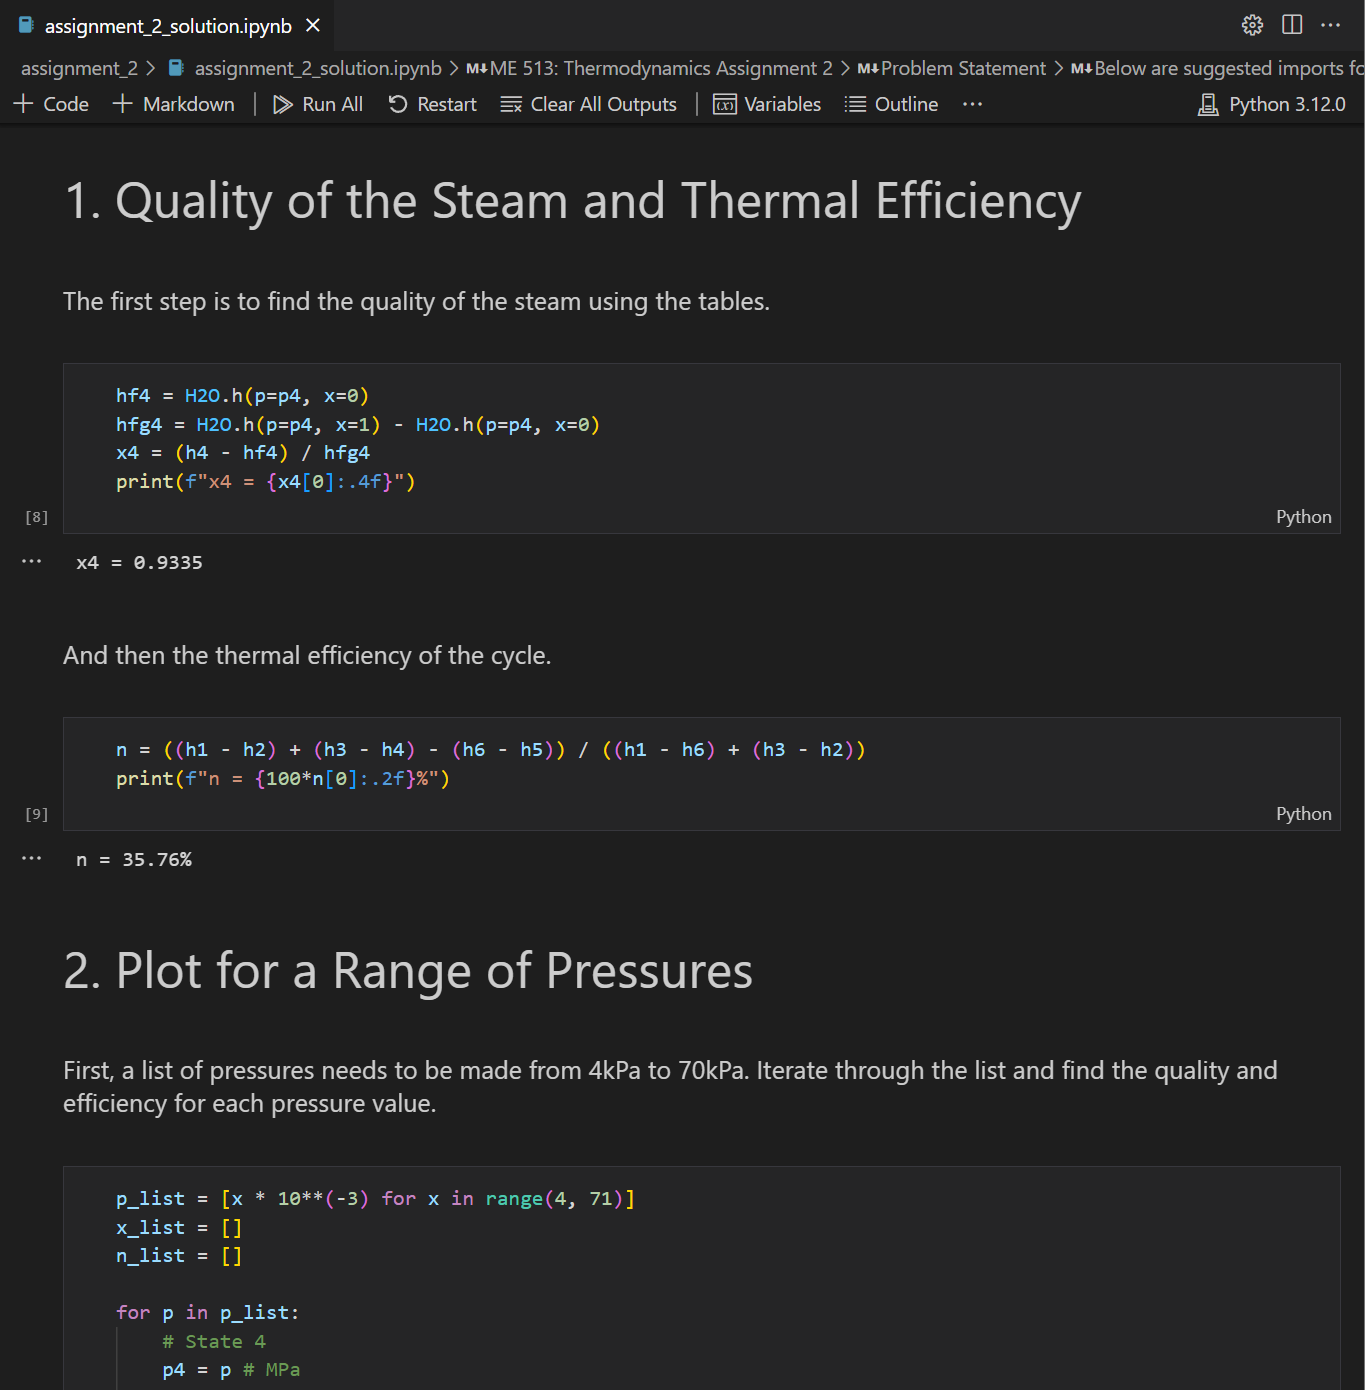
\includegraphics[width=\textwidth]{jupyter-example.png}
    \centering
    \caption{Example of a Jupyter Notebook in VSCode}
    \centering
    \label{fig:jupyter_example}
\end{figure}

The flow provided by Jupyter Notebooks works well, both for giving assignments and
doing in class examples. Jupyter Notebooks also have slideshow capabilities, which allows 
interactive code to fit directly into a lecture presentation without needing to switch between
monitors or tabs.
